\documentclass[12pt,a4paper,openany]{book}
\usepackage{lmodern}
\usepackage[svgnames]{xcolor} % Required to specify font color
\usepackage{xcolor}
\definecolor{vert1}{rgb}{0.0,0.3.9,0.0}
\definecolor{bleu}{rgb}{0,0,0.5}
\definecolor{bleu3}{rgb}{1,0.2,0.2}
\definecolor{grisgris}{gray}{0.4}
\definecolor{grisclair}{HTML}{E7E7E7}
\definecolor{grisfonce}{HTML}{A5A5A5}
\definecolor{rougeUPS}{rgb}{0.6, 0.3, 0.3}

\fboxsep =0pt \parindent =0pt\parskip =12pt



\usepackage[utf8]{inputenc} 
\usepackage[T1]{fontenc}
\usepackage[francais]{babel}
\usepackage[top=1.7cm, bottom=1.7cm, left=1.7cm, right=1.7cm]{geometry}
\usepackage{verbatim}
\usepackage[urlbordercolor={1 1 1}, linkbordercolor={1 1 1}, linkcolor=vert1, urlcolor=bleu, colorlinks=true]{hyperref}
\usepackage{tikz} %Vectoriel
\usepackage{listings}
\usepackage{fancyhdr}
\usepackage{multido}
\usepackage{amssymb}
\usepackage{float}
\usepackage[francais]{minitoc}
\usepackage[final]{pdfpages} 
\usepackage{graphicx} % Required for box manipulation

\newcommand{\titre}{Réseau}
\newcommand{\subtitle}{~}
\newcommand{\auteur}{Antoine de \bsc{Roquemaurel}}
\newcommand{\formation}{L3 Informatique}
\newcommand{\semestre}{5}
\newcommand{\annee}{2013}
\newcommand{\prof}{Jean-Marc \bsc{Pierson} -- Michelle \bsc{Sibilla}}


\newcommand{\pole}{}
\newcommand{\sigle}{reseau}


\definecolor{gris1}{gray}{0.40}
\definecolor{gris2}{gray}{0.55}
\definecolor{gris3}{gray}{0.65}
\definecolor{gris4}{gray}{0.50}
\definecolor{vert}{rgb}{0,0.4,0}
\definecolor{violet}{rgb}{0.65, 0.2, 0.65}
\definecolor{bleu1}{rgb}{0,0,0.8}
\definecolor{bleu2}{rgb}{0,0.2,0.6}
\definecolor{bleu3}{rgb}{0,0.2,0.2}
\definecolor{rouge}{HTML}{F93928}


\lstdefinelanguage{algo}{%
   morekeywords={%
    %%% couleur 1
		importer, programme, glossaire, fonction, procedure, constante, type, 
	%%% IMPORT & Co.
		si, sinon, alors, fin, tantque, debut, faire, lorsque, fin lorsque, 
		declenche, declencher, enregistrement, tableau, retourne, retourner, =, pour, a,
		/=, <, >, traite,exception, 
	%%% types 
		Entier, Reel, Booleen, Caractere, Réél, Booléen, Caractère,
	%%% types 
		entree, maj, sortie,entrée,
	%%% types 
		et, ou, non,
	},
  sensitive=true,
  morecomment=[l]{--},
  morestring=[b]',
}

\lstset{language=algo,
    %%% BOUCLE, TEST & Co.
      emph={importer, programme, glossaire, fonction, procedure, constante, type},
      emphstyle=\color{bleu2},
    %%% IMPORT & Co.  
	emph={[2]
		si, sinon, alors, fin , tantque, debut, faire, lorsque, fin lorsque, 
		declencher, retourner, et, ou, non,enregistrement, retourner, retourne, 
		tableau, /=, <, =, >, traite,exception, pour, a
	},
      emphstyle=[2]\color{bleu1},
    %%% FONCTIONS NUMERIQUES
      emph={[3]Entier, Reel, Booleen, Caractere, Booléen, Réél, Caractère},
      emphstyle=[3]\color{gris1},
    %%% FONCTIONS NUMERIQUES
      emph={[4]entree, maj, sortie, entrée},	
      emphstyle=[4]\color{gris1},
}
\lstdefinelanguage{wl}{%
   morekeywords={%
    %%% couleur 1
		importer, programme, glossaire, fonction, procedure, constante, type, 
	%%% IMPORT & Co.
		si, sinon, alors, fin, TANTQUE, tantque, FIN, PROCEDURE, debut, faire, lorsque, 
		fin lorsque, declenche, declencher, enregistrement, tableau, retourne, retourner, =, 
		/=, <, >, traite,exception, 
	%%% types 
		Entier, Reel, Booleen, Caractere, Réél, Booléen, Caractère,
	%%% types 
		entree, maj, sortie,entrée,
	%%% types 
		et, ou, non,
	},
  sensitive=true,
  morecomment=[l]{//},
  morestring=[b]',
}

\lstset{language=wl,
    %%% BOUCLE, TEST & Co.
      emph={importer, programme, glossaire, fonction, procedure, constante, type},
      emphstyle=\color{bleu2},
    %%% IMPORT & Co.  
	emph={[2]
		si, sinon, alors, fin , tantque, debut, faire, lorsque, fin lorsque, 
		declencher, retourner, et, ou, non,enregistrement, retourner, retourne, 
		tableau, /=, <, =, >, traite,exception
	},
      emphstyle=[2]\color{bleu1},
    %%% FONCTIONS NUMERIQUES
      emph={[3]Entier, Reel, Booleen, Caractere, Booléen, Réél, Caractère},
      emphstyle=[3]\color{gris1},
    %%% FONCTIONS NUMERIQUES
      emph={[4]entree, maj, sortie, entrée},	
      emphstyle=[4]\color{gris1},
}
\lstdefinelanguage{css}{%
   morekeywords={%
    %%% couleur 1
		background, image, repeat, position, index, color, border, font, 
		size, url, family, style, variant, weight, letter, spacing, line, 
		height, text, decoration, align, indent, transform, shadow, 
		background, image, repeat, position, index, color, border, font, 
		size, url, family, style, variant, weight, letter, spacing, line, 
		height, text, decoration, align, indent, transform, shadow, 
		vertical, align, white, space, word, spacing,attachment, width, 
		max, min, margin, padding, clip, direction, display, overflow,
		visibility, clear, float, top, right, bottom, left, list, type, 
		collapse, side, empty, cells, table, layout, cursor, marks, page, break,
		before, after, inside, orphans, windows, azimuth, after, before, cue, 
		elevation, pause, play, during, pitch, range, richness, spek, header, 
		numeral, punctuation, rate, stress, voice, volume,
	%%% types 
		left, right, bottom, top, none, center, solid, black, blue, red, green,
	},
  sensitive=true,
  sensitive=true,
  morecomment=[s]{/*}{*/},
  morestring=[b]',
}
\lstset{language=css,
    %%% BOUCLE, TEST & Co.
      emph={
		background, image, repeat, position, index, color, border, font, 
		size, url, family, style, variant, weight, letter, spacing, line, 
		height, text, decoration, align, indent, transform, shadow, 
		background, image, repeat, position, index, color, border, font, 
		size, url, family, style, variant, weight, letter, spacing, line, 
		height, text, decoration, align, indent, transform, shadow, 
		vertical, align, white, space, word, spacing,attachment, width, 
		max, min, margin, padding, clip, direction, display, overflow,
		visibility, clear, float, top, right, bottom, left, list, type, 
		collapse, side, empty, cells, table, layout, cursor, marks, page, break,
		before, after, inside, orphans, windows, azimuth, after, before, cue, 
		elevation, pause, play, during, pitch, range, richness, spek, header, 
		numeral, punctuation, rate, stress, voice, volume,
	  },
      emphstyle=\color{bleu2},
    %%% FONCTIONS NUMERIQUES
      emph={[3]
		left, right, bottom, top,none, solid, black, blue, green,
		  },
      emphstyle=[3]\color{bleu3},
    %%% FONCTIONS NUMERIQUES
}

\lstset{language=SQL,
    %%% BOUCLE, TEST & Co.
      emph={INSERT, UPDATE, DELETE, WHERE, SET, GROUP, BY, ORDER, REFERENCES},
      emphstyle=\color{bleu2},
    %%% IMPORT & Co.  
	emph={[2]
		if, end, begin, then, for, each, else, after, of, on, to
	},
      emphstyle=[2]\color{bleu1},
    %%% FONCTIONS NUMERIQUES
      emph={[3]Entier, Reel, Booleen, Caractere, Booléen, Réél, Caractère},
      emphstyle=[3]\color{gris1},
    %%% FONCTIONS NUMERIQUES
      emph={[4]entree, maj, sortie, entrée},	
      emphstyle=[4]\color{gris1},
}
\lstdefinelanguage{ARM}{%
   morekeywords={%
   ADD, SUB, MOV, MUL, RSB,CMP, BLS, BLE, B,BHI,LDR,
   BGE, RSBLT, BGT, BEQ, BNE,BLT,BHS,STR,STRB
	},
  sensitive=true,
  morecomment=[l]{@},
  morestring=[b]',
}

\lstset{ % general style for listings 
   numbers=left 
   , literate={é}{{\'e}}1 {è}{{\`e}}1 {à}{{\`a}}1 {ê}{{\^e}}1 {É}{{\'E}}1 {ô}{{\^o}}1 {€}{{\euro}}1{°}{{$^{\circ}$}}1 {ç}{ {c}}1 {ù}{u}1
	, extendedchars=\true
   , tabsize=2 
   , frame=l
   , framerule=1.1pt
   , linewidth=520px
   , breaklines=true 
   , basicstyle=\footnotesize\ttfamily 
   , numberstyle=\tiny\ttfamily 
   , framexleftmargin=0mm 
   , xleftmargin=0mm 
   , captionpos=b 
	, keywordstyle=\color{bleu2}
	, commentstyle=\color{vert}
	, stringstyle=\color{rouge}
	, showstringspaces=false
	, extendedchars=true
	, mathescape=true
} 
%	\lstlistoflistings
%	\addcontentsline{toc}{part}{List of code examples}

\documentclass[12pt,a4paper,openany]{book}
\usepackage{lmodern}
\usepackage{xcolor}
\usepackage{xcolor}
\definecolor{vert1}{rgb}{0.0,0.3.9,0.0}
\definecolor{bleu}{rgb}{0,0,0.5}
\definecolor{bleu3}{rgb}{1,0.2,0.2}
\definecolor{grisgris}{gray}{0.4}
\definecolor{grisclair}{HTML}{E7E7E7}
\definecolor{grisfonce}{HTML}{A5A5A5}
\definecolor{rougeUPS}{rgb}{0.6, 0.3, 0.3}

\fboxsep =0pt \parindent =0pt\parskip =12pt



\usepackage[utf8]{inputenc}
\usepackage[T1]{fontenc}
\usepackage[francais]{babel}
\usepackage[top=1.7cm, bottom=1.7cm, left=1.7cm, right=1.7cm]{geometry}
\usepackage{verbatim}
\usepackage[urlbordercolor={1 1 1}, linkbordercolor={1 1 1}, linkcolor=vert1, urlcolor=bleu, colorlinks=true]{hyperref}
\usepackage{tikz} %Vectoriel
\usepackage{listings}
\usepackage{fancyhdr}
\usepackage{multido}
\usepackage{amssymb}
\usepackage{float}

\newcommand{\titre}{Complexité des algorithmes}

\newcommand{\pole}{}
\newcommand{\sigle}{complexite}

\newcommand{\semestre}{3}

\definecolor{gris1}{gray}{0.40}
\definecolor{gris2}{gray}{0.55}
\definecolor{gris3}{gray}{0.65}
\definecolor{gris4}{gray}{0.50}
\definecolor{vert}{rgb}{0,0.4,0}
\definecolor{violet}{rgb}{0.65, 0.2, 0.65}
\definecolor{bleu1}{rgb}{0,0,0.8}
\definecolor{bleu2}{rgb}{0,0.2,0.6}
\definecolor{bleu3}{rgb}{0,0.2,0.2}
\definecolor{rouge}{HTML}{F93928}


\lstdefinelanguage{algo}{%
   morekeywords={%
    %%% couleur 1
		importer, programme, glossaire, fonction, procedure, constante, type, 
	%%% IMPORT & Co.
		si, sinon, alors, fin, tantque, debut, faire, lorsque, fin lorsque, 
		declenche, declencher, enregistrement, tableau, retourne, retourner, =, pour, a,
		/=, <, >, traite,exception, 
	%%% types 
		Entier, Reel, Booleen, Caractere, Réél, Booléen, Caractère,
	%%% types 
		entree, maj, sortie,entrée,
	%%% types 
		et, ou, non,
	},
  sensitive=true,
  morecomment=[l]{--},
  morestring=[b]',
}

\lstset{language=algo,
    %%% BOUCLE, TEST & Co.
      emph={importer, programme, glossaire, fonction, procedure, constante, type},
      emphstyle=\color{bleu2},
    %%% IMPORT & Co.  
	emph={[2]
		si, sinon, alors, fin , tantque, debut, faire, lorsque, fin lorsque, 
		declencher, retourner, et, ou, non,enregistrement, retourner, retourne, 
		tableau, /=, <, =, >, traite,exception, pour, a
	},
      emphstyle=[2]\color{bleu1},
    %%% FONCTIONS NUMERIQUES
      emph={[3]Entier, Reel, Booleen, Caractere, Booléen, Réél, Caractère},
      emphstyle=[3]\color{gris1},
    %%% FONCTIONS NUMERIQUES
      emph={[4]entree, maj, sortie, entrée},	
      emphstyle=[4]\color{gris1},
}
\lstdefinelanguage{wl}{%
   morekeywords={%
    %%% couleur 1
		importer, programme, glossaire, fonction, procedure, constante, type, 
	%%% IMPORT & Co.
		si, sinon, alors, fin, TANTQUE, tantque, FIN, PROCEDURE, debut, faire, lorsque, 
		fin lorsque, declenche, declencher, enregistrement, tableau, retourne, retourner, =, 
		/=, <, >, traite,exception, 
	%%% types 
		Entier, Reel, Booleen, Caractere, Réél, Booléen, Caractère,
	%%% types 
		entree, maj, sortie,entrée,
	%%% types 
		et, ou, non,
	},
  sensitive=true,
  morecomment=[l]{//},
  morestring=[b]',
}

\lstset{language=wl,
    %%% BOUCLE, TEST & Co.
      emph={importer, programme, glossaire, fonction, procedure, constante, type},
      emphstyle=\color{bleu2},
    %%% IMPORT & Co.  
	emph={[2]
		si, sinon, alors, fin , tantque, debut, faire, lorsque, fin lorsque, 
		declencher, retourner, et, ou, non,enregistrement, retourner, retourne, 
		tableau, /=, <, =, >, traite,exception
	},
      emphstyle=[2]\color{bleu1},
    %%% FONCTIONS NUMERIQUES
      emph={[3]Entier, Reel, Booleen, Caractere, Booléen, Réél, Caractère},
      emphstyle=[3]\color{gris1},
    %%% FONCTIONS NUMERIQUES
      emph={[4]entree, maj, sortie, entrée},	
      emphstyle=[4]\color{gris1},
}
\lstdefinelanguage{css}{%
   morekeywords={%
    %%% couleur 1
		background, image, repeat, position, index, color, border, font, 
		size, url, family, style, variant, weight, letter, spacing, line, 
		height, text, decoration, align, indent, transform, shadow, 
		background, image, repeat, position, index, color, border, font, 
		size, url, family, style, variant, weight, letter, spacing, line, 
		height, text, decoration, align, indent, transform, shadow, 
		vertical, align, white, space, word, spacing,attachment, width, 
		max, min, margin, padding, clip, direction, display, overflow,
		visibility, clear, float, top, right, bottom, left, list, type, 
		collapse, side, empty, cells, table, layout, cursor, marks, page, break,
		before, after, inside, orphans, windows, azimuth, after, before, cue, 
		elevation, pause, play, during, pitch, range, richness, spek, header, 
		numeral, punctuation, rate, stress, voice, volume,
	%%% types 
		left, right, bottom, top, none, center, solid, black, blue, red, green,
	},
  sensitive=true,
  sensitive=true,
  morecomment=[s]{/*}{*/},
  morestring=[b]',
}
\lstset{language=css,
    %%% BOUCLE, TEST & Co.
      emph={
		background, image, repeat, position, index, color, border, font, 
		size, url, family, style, variant, weight, letter, spacing, line, 
		height, text, decoration, align, indent, transform, shadow, 
		background, image, repeat, position, index, color, border, font, 
		size, url, family, style, variant, weight, letter, spacing, line, 
		height, text, decoration, align, indent, transform, shadow, 
		vertical, align, white, space, word, spacing,attachment, width, 
		max, min, margin, padding, clip, direction, display, overflow,
		visibility, clear, float, top, right, bottom, left, list, type, 
		collapse, side, empty, cells, table, layout, cursor, marks, page, break,
		before, after, inside, orphans, windows, azimuth, after, before, cue, 
		elevation, pause, play, during, pitch, range, richness, spek, header, 
		numeral, punctuation, rate, stress, voice, volume,
	  },
      emphstyle=\color{bleu2},
    %%% FONCTIONS NUMERIQUES
      emph={[3]
		left, right, bottom, top,none, solid, black, blue, green,
		  },
      emphstyle=[3]\color{bleu3},
    %%% FONCTIONS NUMERIQUES
}

\lstset{language=SQL,
    %%% BOUCLE, TEST & Co.
      emph={INSERT, UPDATE, DELETE, WHERE, SET, GROUP, BY, ORDER, REFERENCES},
      emphstyle=\color{bleu2},
    %%% IMPORT & Co.  
	emph={[2]
		if, end, begin, then, for, each, else, after, of, on, to
	},
      emphstyle=[2]\color{bleu1},
    %%% FONCTIONS NUMERIQUES
      emph={[3]Entier, Reel, Booleen, Caractere, Booléen, Réél, Caractère},
      emphstyle=[3]\color{gris1},
    %%% FONCTIONS NUMERIQUES
      emph={[4]entree, maj, sortie, entrée},	
      emphstyle=[4]\color{gris1},
}
\lstdefinelanguage{ARM}{%
   morekeywords={%
   ADD, SUB, MOV, MUL, RSB,CMP, BLS, BLE, B,BHI,LDR,
   BGE, RSBLT, BGT, BEQ, BNE,BLT,BHS,STR,STRB
	},
  sensitive=true,
  morecomment=[l]{@},
  morestring=[b]',
}

\lstset{ % general style for listings 
   numbers=left 
   , literate={é}{{\'e}}1 {è}{{\`e}}1 {à}{{\`a}}1 {ê}{{\^e}}1 {É}{{\'E}}1 {ô}{{\^o}}1 {€}{{\euro}}1{°}{{$^{\circ}$}}1 {ç}{ {c}}1 {ù}{u}1
	, extendedchars=\true
   , tabsize=2 
   , frame=l
   , framerule=1.1pt
   , linewidth=520px
   , breaklines=true 
   , basicstyle=\footnotesize\ttfamily 
   , numberstyle=\tiny\ttfamily 
   , framexleftmargin=0mm 
   , xleftmargin=0mm 
   , captionpos=b 
	, keywordstyle=\color{bleu2}
	, commentstyle=\color{vert}
	, stringstyle=\color{rouge}
	, showstringspaces=false
	, extendedchars=true
	, mathescape=true
} 
%	\lstlistoflistings
%	\addcontentsline{toc}{part}{List of code examples}
 %prise en charge du langage C 
\date{\today}

\makeindex
\lfoot{Université Toulouse III -- Paul Sabatier}
\rfoot{\sigle\semestre}
%\rfoot{}
\cfoot{}
\makeglossary
\makeatletter
\def\clap#1{\hbox to 0pt{\hss #1\hss}}%
\def\ligne#1{%
\hbox to \hsize{%
\vbox{\centering #1}}}%
\def\haut#1#2#3{%
\hbox to \hsize{%
\rlap{\vtop{\raggedright #1}}%
\hss
\clap{\vtop{\centering #2}}%
\hss
\llap{\vtop{\raggedleft #3}}}}%
\def\bas#1#2#3{%
\hbox to \hsize{%
\rlap{\vbox{\raggedright #1}}%
\hss \clap{\vbox{\centering #2}}%
\hss
\llap{\vbox{\raggedleft #3}}}}%
\def\maketitle{%
\thispagestyle{empty}\vbox to \vsize{%
\haut{}{\@blurb}{}

\vfill
\vspace{1cm}
\begin{flushleft}
\usefont{OT1}{ptm}{m}{n}
\huge \@title
\end{flushleft}
\par
\hrule height 4pt
\par
\begin{flushright}
\usefont{OT1}{phv}{m}{n}
\Large \@author
\par
\end{flushright}
\vspace{1cm}
\vfill
\vfill
\bas{}{\@location, le \@date}{}
}%
\cleardoublepage
}
\def\date#1{\def\@date{#1}}
\def\author#1{\def\@author{#1}}
\def\title#1{\def\@title{#1}}
\def\location#1{\def\@location{#1}}
\def\blurb#1{\def\@blurb{#1}}
\date{\today}
\author{}
\title{}
\location{Amiens}\blurb{}
\makeatother
\title{\titre}
\author{Semestre \semestre}

\location{Toulouse}
\blurb{%
Université Toulouse III -- Paul sabatier\\
L2 Informatique\\
}%



%\title{Cours \\ \titre}
%\date{\today\\ Semestre \semestre}

%\lhead{Cours: \titre}
%\chead{}
%\rhead{\thepage}

%\lfoot{Université Paul Sabatier Toulouse III}
%\cfoot{\thepage}
%\rfoot{\sigle\semestre}

\pagestyle{fancy}
\renewcommand{\chaptermark}[1]{\markboth{\bsc{\chaptername~\thechapter{} :} #1}{}}
\renewcommand{\sectionmark}[1]{\markright{\thesection{ #1}}}
\renewcommand{\headrulewidth}{0.3pt}
\renewcommand{\footrulewidth}{0.3pt}

\fancyhf{}
\fancyhead[LE]{\leftmark}
\fancyhead[RO]{\rightmark}
\fancyfoot[LE,RO]{--~\thepage~--}
\fancyfoot[LO]{\titre{}~~---~~\sigle{}\semestre{}}
\fancyfoot[RE]{Antoine de \bsc{Roquemaurel}}

%% Cas des premières pages de chapitre
\fancypagestyle{plain}{%
	\fancyhf{}%
	\fancyfoot[L]{\titre{}~~---~~\sigle{}\semestre{}}
	\fancyfoot[R]{--~\thepage~--}
	\renewcommand{\headrulewidth}{0pt}
	\renewcommand{\footrulewidth}{0.3pt}
}
\makeatletter
\renewcommand*{\lstlistlistingname}{Liste des codes sources}
\renewcommand\listoffigures{%
    \chapter{\listfigurename}%
      \@mkboth{\MakeUppercase\listfigurename}%
              {\MakeUppercase\listfigurename}%
       \@starttoc{lof}%
    }
    \renewcommand\listoftables{%
    \chapter{\listtablename}%
    \@mkboth{\MakeUppercase{\listtablename}}%
            {\MakeUppercase{\listtablename}}%
    \@starttoc{lot}
    }

    \renewcommand\lstlistoflistings{%
    \begingroup
    \chapter{\lstlistlistingname}%
    \parskip\z@\parindent\z@\parfillskip \z@ \@plus 1fil%
    \@starttoc{lol}%
    \endgroup
    }
	\makeatother

\newcommand{\remarque}[1]{
	\begin{center}
	\medskip
	\colorbox{remarque}{
		\begin{minipage}{0.85\textwidth}\medskip
\includegraphics[height=10px]{images/remarque.png} #1 \medskip\end{minipage}
	}
	\medskip
	\end{center}
}

\newcounter{exemples}

\newenvironment{exemple}[1]{
   \vspace{-2mm}

\refstepcounter{exemples}
   \begin{center}
	\medskip
      \begin{minipage}{0.9\linewidth}
}{%
~
      \end{minipage}
   \end{center}~
   \vspace{-2mm}
}%

\newcommand{\captionExemple}[1]{
	\begin{center}{\bsc{Exemple} \thechapter.\arabic{exemples}~--~}#1\end{center}
}

\DeclareTextFontCommand{\policeGlossaire}{\fontfamily{lmss}\selectfont}
\DeclareTextFontCommand{\policePackage}{\fontfamily{phv}\selectfont}
\DeclareTextFontCommand{\policeTitre}{\fontfamily{ptm}\selectfont}
\newcommand{\policeCode}[1]{\texttt{#1}}

\newcommand{\sectionfont}{%
	\fontencoding{\encodingdefault}%
	\fontfamily{pag}%
	\fontseries{bc}%
	\fontshape{n}%
	\selectfont
}

% numéro du chapitre
\DeclareFixedFont{\chapnumfont}{T1}{phv}{b}{n}{80pt}
% pour le mot « Chapitre »
\DeclareFixedFont{\chapchapfont}{T1}{phv}{b}{n}{16pt}
% pour le titre
\DeclareFixedFont{\chaptitfont}{T1}{phv}{b}{n}{24.88pt}


\makeatletter
\def\thickhrulefill{\leavevmode \leaders \hrule height 1ex \hfill \kern \z@}
%% \chapter
\def\@makechapterhead#1{%
  \reset@font
  \parindent \z@
  \vspace*{10\p@}%
  \hbox{%
    \vbox{%
      \advance\hsize by -2cm
      \hrule height 0.4pt depth 0pt width \hsize
      \par
      \vskip 6pt%
      \hspace{20pt}%
      \parbox{420pt}{%
        \LARGE \bfseries #1
		}%
      \par
      \vskip 6pt%
      \hspace{20pt}%
      \hrule height 0.4pt depth 0pt width \hsize
	  \vspace{-30pt}
      }%
    \vbox{%
      \hsize=1.5cm%
      \begin{tabular}{c}
        \scshape \large \strut \@chapapp{} \\
        \colorbox{black}{\vbox{\hbox{\vbox to 1mm{}}\hbox{
			\color{white} \LARGE \bfseries \hspace{1mm}\thechapter\hspace{1mm}
		}\hbox{\vbox to 2cm{}}}}%
      \end{tabular}%
      }%
    }%
  \vskip 20\p@
}
%% \chapter*
\def\@makeschapterhead#1{%
  \reset@font
  \parindent \z@
  \vspace*{10\p@}%
  \hbox{%
    \vbox{%
      \advance\hsize by -0cm
      \hrule height 0.4pt depth 0pt width \hsize
      \par
      \vskip 6pt%
      \hspace{20pt}%
      \parbox{420pt}{%
        \LARGE \bfseries #1
		}%
      \par
      \vskip 6pt%
      \hspace{20pt}%
      \hrule height 0.4pt depth 0pt width \hsize
      }%
    }%
  \vskip 20\p@

}

\newlength{\sectiontitleindent}
\newlength{\subsectiontitleindent}
\newlength{\subsubsectiontitleindent}
\setlength{\sectiontitleindent}{-1cm}
\setlength{\subsectiontitleindent}{-.5cm}
\setlength{\subsubsectiontitleindent}{-.25cm}

\renewcommand{\section}{%
	\@startsection%
	{section}%
	{1}%
	{\sectiontitleindent}%
	{-3.5ex plus -1ex minus -.2ex}%
	{2.3ex plus.2ex}%
	{\sectionfont\Large}
}
\renewcommand{\subsection}{%
	\@startsection%
	{subsection}%
	{2}%
	{\subsectiontitleindent}%
	{-3.5ex plus -1ex minus -.2ex}%
	{2.3ex plus.2ex}%
	{\sectionfont\large}
}

\renewcommand{\subsubsection}{%
	\@startsection%
	{subsubsection}%
	{3}%
	{\subsubsectiontitleindent}%
	{-3.5ex plus -1ex minus -.2ex}%
	{2.3ex plus.2ex}%
	{\sectionfont\normalsize}
}

\makeatother



\newcommand{\pfp}{\texttt{pfp}}

\newcommand{\ifp}{\texttt{if}}
\newcommand{\moy}{\textrm{moy}}
\newcommand{\prob}{\textrm{prob}}
\newcommand{\elsep}{\texttt{else}}

\makeatother

\begin{document}
	\setcounter{tocdepth}{1}
	\setcounter{secnumdepth}{3}
	\maketitle
	\tableofcontents
	\chapter{Introduction}
		\section{Complexité}
		On cherche à estimer le temps de calcul d'un algorithme A en fonction d'un paramètre n. Pour avoir une mesure indépendante de la machine, on identifie
		le temps de calcul avec le nombre d'instructions exécutées. 
		
		\exemple{Le paramètre n pourrait être la taille d'un tableau, par exemple.}

		Soit $D_i$ l'ensemble des données possibles telle que $n=i$. Pour $d \in D_i$ on notera $T(A,d)$ le nombre d'instructions exécutée pendant l'exécution de
		$A(d)$.\\
		On notera $\prob(d|i)$ la probabilité que les données soit $d$ étant donné qu'elles sont de taille $i$.

		\subsection{La complexité temporelle maximale} 
		La complexité temporelle maximale\footnote{Complexité dans le pire des cas} d'un algorithme A :
		$$T_{\max}(i) = \max_{d\in D_i}\{T(A,d)\}$$
		\subsection{La complexité temporelle moyenne}
		La complexité temporelle moyenne\footnote{Complexité dans le cas moyen} d'un algorithme A :
		$$T_{\moy} = \sum_{d \in D_i} \prob(d|i) \times T(A,d)$$
		\remarque{Pour pouvoir calculer $T_\moy$, il faut connaître la distribution des données, ce qui n'est pas toujours évident (par exemple en traitement d'image)}
		\subsection{La complexité temporelle minimale}
		La complexité temporelle minimale\footnote{Complexité dans le meilleur des cas} d'un algorithme A :
		$$T_{\min}(i) = \min_{d\in D_i}\{T(A,d)\}$$ 
		\remarque{Peu utilisé, sauf pour prouver qu'un algorithme est mauvais. Si la complexité temporelle minimale est 
			mauvaise même dans le meilleur des cas, alors l'algorithme n'est pas bon.}

%			\remarque{$T_{\max}$ et $T_{\min}$ nous fournissent des bornes supérieures et inférieures.}

		\subsection{Compairaison de complexités en fonction de la machine}
		\begin{tabular}{| c | p{7cm} | p{7cm}|} 
			\hline
			\textbf{Complexité}& \multicolumn{2}{|c|}{\textbf{Nombre d'instructions pouvant executer la machine}}\\
			\hline
			 & $1\;000\;000$ & $1\;000\;000\;000\;000$\\
			\hline
			$n$ & $1\;000\;000$&$1\;000\;000\;000\;000$\\
			\hline
			$n \log_2 n$ &$64\;000$&$32\;000\;000\;000$\\
			\hline
			$n^2$ & $1\;000$&$1\;000\;000$\\
			\hline
			$n^3$ &$100$&$10\;000$\\
			\hline
			$2^n$ &$20$&$40$\\
			\hline
		\end{tabular}
		\section{Complexité asymptotique}
		Pour comparer des algorithmes, on ne s'intéresse qu'à leur comportements pour n grand. On cherche une mesure de complexité qui soit indépendante du langage de programmation et de la vitesse de la machine. \\ 
	$\Rightarrow$		On ne doit pas perdre en compte des facteurs constants.  \\
	$\Rightarrow$	Ordre de grandeur

	\subsection{La complexité asymptotique}
	La complexité asymptotique\footnote{Que ce soit maximale, moyenne ou minimale} est l'ordre de grandeur de sa limite lorsque $n \rightarrow \infty$

	\subsection{Notation} Soient $T$, $f$ des fonctions positives ou nulles. Rotations de grandeur de fonction asymptotiques.
	\paragraph{Grand O} $T = O(f)$ si $\exists c \in \mathbb{R}^{>0}$ et $n_0 \in \mathbb{N}$ tels que $\forall n \geq n_0$, $T(n) \leq cf(n)$.

	\paragraph{Grand Oméga} $T = \Omega(f)$ si $\exists c \in \mathbb{R}^{>0}$ et $n_0 \in \mathbb{N}$ tels que $i\forall n \geq n_0$, $T(n) \geq cf(n)$
	\paragraph{Petit O} $T = o(f)$ si $\frac{T(n)}{f(n)} \rightarrow O$ lorsque $n \rightarrow \infty$. 
	\remarque{T est négligeable devant f}

	\exemple{
	\begin{enumerate}
		\item $2n^2 + 5n + 10 = O(n^2)$\\
		Dans la définition $n_0 = 5$,$c=4$ : \\
		$\forall n \geq 5,\ 2n^2+5n+10 \leq 4n^2$
	\item $2n^2 + 5n + 10 = \Omega(n^2)$\\
		Dans la définition, $n_0 = 1$, $c = 2$\\
		$\forall n \geq 1,\ 2n^2 + 5n + 10 \geq 2n^2 \cdots$\\
		Donc $2n^2+5n+10 = \Theta (n^2)$
	\item $\frac{1}{5} + n = O(n\log_2 n)\ (n_0 = 2,\ c=2)$
	\item $\frac{1}{5} n \log_2 n + n = \Omega(n \log n)\ (n_0=1,c=\frac{1}{5})$
	\item $\forall k \geq 0$, $n^k = O(n^{k+1})$ mais $n^k \neq \Omega(n^{k+1})$
	\item $\forall a,b >1, \log_a n = \Theta (\log_b n)$ car $\log_a n = \frac{\log_b n}{\log_b a}$ et $\log_b a$ est une constante. $\Rightarrow$ On a pas besoin de préciser la base de logarithme dnas une complexité asymptotique
	\item $2n^2 + 5n + 10 = 2n^2 + 0(n^2)$
	\item Pour toute constante $c>0$, $C = \Theta(1)$
	\item $2^n = o(3^n)$
	\end{enumerate}
	}
	\remarque{\begin{enumerate}
		\item O et $\Omega$ sont des pré-ordres\footnote{Relations reflexives et transitives} :\\ $f = O(f)$ et $f = O(g)$ et $g = O(h)) \Rightarrow f = O(h)$
		\item $\Theta$ est une relation d'équivalence\footnote{relation reflexives, symétrique et transitive} : 
			$f = \Theta(g) \Leftrightarrow g = \Theta (f)$
	\end{enumerate}
	}
	\paragraph{Proposition}
	$$\textrm{Si } \lim_{n \rightarrow \infty} \frac{f(n)}{g(n)} = a > 0 \textrm{ Alors }f = \Theta (g)$$
	\remarque{La réciproque est fausse}

	\paragraph{Notation} $$f \sim g \Rightarrow \lim_{n\rightarrow \infty} \frac{f(n)}{g(n)} = 1$$
	\exemple{$(3n+1)^3 \sim 27n^3$}
	\section{Exemple de complexités d'algorithmes}
	\subsection{Le tri à bulles}
	\begin{eqnarray*}
		T_{\min} (n) &=& \Theta (n) \textrm{ Si le tableau est est déjà trié}\\
		T_{\max}(n) &=& \Theta(n^2) \textrm{ Si le tableau est trié en ordre décroissant}\\
		T_{\moy}(n) &=& T_{\max}(n) = \Theta(n^2)\\
	\end{eqnarray*}
	\subsection{Tri par fusion}
	\begin{eqnarray*}
		T_{\min}(n) = T_{\max}(n) = T_{\moy}(n) = \Theta (n\log n)
	\end{eqnarray*}
	\subsection{Tri rapide}
	\begin{eqnarray*}
		T_{\min}(n) = T_{\moy}(n) &=& \Theta (n \log n)\\
		T_{\max}(n) &=& \Theta(n^2)
	\end{eqnarray*}
	\chapter{Complexité des boucles}
	\chapter{Complexité d'algorithmes définis par réccurence}
	\chapter{Structure de données et complexité}
	
	\appendix
	\chapter{Exercices}
	\section{TD 1}
\end{document}



\newcommand{\remarque}[1]{
	\begin{center}
	\medskip
	\colorbox{remarque}{
		\begin{minipage}{0.85\textwidth}\medskip
\includegraphics[height=10px]{images/remarque.png} #1 \medskip\end{minipage}
	}
	\medskip
	\end{center}
}

\newcounter{exemples}

\newenvironment{exemple}[1]{
   \vspace{-2mm}

\refstepcounter{exemples}
   \begin{center}
	\medskip
      \begin{minipage}{0.9\linewidth}
}{%
~
      \end{minipage}
   \end{center}~
   \vspace{-2mm}
}%

\newcommand{\captionExemple}[1]{
	\begin{center}{\bsc{Exemple} \thechapter.\arabic{exemples}~--~}#1\end{center}
}

\DeclareTextFontCommand{\policeGlossaire}{\fontfamily{lmss}\selectfont}
\DeclareTextFontCommand{\policePackage}{\fontfamily{phv}\selectfont}
\DeclareTextFontCommand{\policeTitre}{\fontfamily{ptm}\selectfont}
\newcommand{\policeCode}[1]{\texttt{#1}}

\newcommand{\sectionfont}{%
	\fontencoding{\encodingdefault}%
	\fontfamily{pag}%
	\fontseries{bc}%
	\fontshape{n}%
	\selectfont
}

% numéro du chapitre
\DeclareFixedFont{\chapnumfont}{T1}{phv}{b}{n}{80pt}
% pour le mot « Chapitre »
\DeclareFixedFont{\chapchapfont}{T1}{phv}{b}{n}{16pt}
% pour le titre
\DeclareFixedFont{\chaptitfont}{T1}{phv}{b}{n}{24.88pt}


\makeatletter
\def\thickhrulefill{\leavevmode \leaders \hrule height 1ex \hfill \kern \z@}
%% \chapter
\def\@makechapterhead#1{%
  \reset@font
  \parindent \z@
  \vspace*{10\p@}%
  \hbox{%
    \vbox{%
      \advance\hsize by -2cm
      \hrule height 0.4pt depth 0pt width \hsize
      \par
      \vskip 6pt%
      \hspace{20pt}%
      \parbox{420pt}{%
        \LARGE \bfseries #1
		}%
      \par
      \vskip 6pt%
      \hspace{20pt}%
      \hrule height 0.4pt depth 0pt width \hsize
	  \vspace{-30pt}
      }%
    \vbox{%
      \hsize=1.5cm%
      \begin{tabular}{c}
        \scshape \large \strut \@chapapp{} \\
        \colorbox{black}{\vbox{\hbox{\vbox to 1mm{}}\hbox{
			\color{white} \LARGE \bfseries \hspace{1mm}\thechapter\hspace{1mm}
		}\hbox{\vbox to 2cm{}}}}%
      \end{tabular}%
      }%
    }%
  \vskip 20\p@
}
%% \chapter*
\def\@makeschapterhead#1{%
  \reset@font
  \parindent \z@
  \vspace*{10\p@}%
  \hbox{%
    \vbox{%
      \advance\hsize by -0cm
      \hrule height 0.4pt depth 0pt width \hsize
      \par
      \vskip 6pt%
      \hspace{20pt}%
      \parbox{420pt}{%
        \LARGE \bfseries #1
		}%
      \par
      \vskip 6pt%
      \hspace{20pt}%
      \hrule height 0.4pt depth 0pt width \hsize
      }%
    }%
  \vskip 20\p@

}

\newlength{\sectiontitleindent}
\newlength{\subsectiontitleindent}
\newlength{\subsubsectiontitleindent}
\setlength{\sectiontitleindent}{-1cm}
\setlength{\subsectiontitleindent}{-.5cm}
\setlength{\subsubsectiontitleindent}{-.25cm}

\renewcommand{\section}{%
	\@startsection%
	{section}%
	{1}%
	{\sectiontitleindent}%
	{-3.5ex plus -1ex minus -.2ex}%
	{2.3ex plus.2ex}%
	{\sectionfont\Large}
}
\renewcommand{\subsection}{%
	\@startsection%
	{subsection}%
	{2}%
	{\subsectiontitleindent}%
	{-3.5ex plus -1ex minus -.2ex}%
	{2.3ex plus.2ex}%
	{\sectionfont\large}
}

\renewcommand{\subsubsection}{%
	\@startsection%
	{subsubsection}%
	{3}%
	{\subsubsectiontitleindent}%
	{-3.5ex plus -1ex minus -.2ex}%
	{2.3ex plus.2ex}%
	{\sectionfont\normalsize}
}

\makeatother



\newcommand{\pfp}{\texttt{pfp}}

\newcommand{\ifp}{\texttt{if}}
\newcommand{\elsep}{\texttt{else}}

\usepackage{ifthen}

\newsavebox{\fmbox}
\newenvironment{fmpage}[1]
     {\begin{lrbox}{\fmbox}\begin{minipage}{#1}}
	  {\end{minipage}\end{lrbox}\fbox{\usebox{\fmbox}}}


\makeatletter

\title{Projet Agile --- \bsc{SCRUM}}

\def\top#1{\def\@top{#1}}

\def\sousTitre#1{\def\@sousTitre{#1}}
\sousTitre{Rubidium}

\def\location#1{\def\@location{#1}}
\location{Toulouse}

\date{\today}

%% Entete (Université..)  
\def\clap#1{
	\hbox to 0pt{\hss #1\hss}
}%
\def\ligne#1{%
	\hbox to \hsize{%
		\vbox{\centering #1}
	}
}%

% définition du haut de la couverture %
\def\haut#1#2#3{%
	\hbox to \hsize{%
		\rlap{
			\vtop{\raggedright #1}
		}%
		\hss
		\clap{	
			\vtop{\centering #2}
		}%
		\hss
		\llap{
			\vtop{\raggedleft #3}
		}
	}
}%

% Définition du bas de la couverture %
\def\bas#1#2#3{%
	\hbox to \hsize{%
	\hss \clap{\vbox{
	\centering \hspace{1.7cm}\newline
		\newline \newline \newline	\newline \newline \newline	\newline \newline \newline	\newline \newline \newline	\newline \newline \newline	\newline \newline \newline\newline #2 }
		}%
		\hss
	}
}%

% Zou, on peut construire la page de garde 
\def\maketitle{%
	\thispagestyle{empty}\vbox to \vsize{%
		\vspace{-25px}
		\vspace{5px}
		\haut{}{\@top}{}
		\vfill
		\begin{flushleft}
			David \bsc{Bernard}\\
			Mathias \bsc{Faure}\\
			Antoine \bsc{Incorvaia}\\
			Lucas \bsc{Le gouic}\\
			Antoine de \bsc{Roquemaurel}\\
			Clément \bsc{Vannier}\\
		\end{flushleft}

		\begin{flushright}
			\vspace{-3cm}
			\begin{tabular}{r@{~}l}
				Pour M. \bsc{Fernandez} 
			\end{tabular}
		\end{flushright}
		\vfill
		\vspace{1cm}
		\begin{flushleft}
			\policeTitre{\huge \@title}
		\end{flushleft}

		\par
		\hrule height 4pt
		\par

		\begin{flushright}
			\policeTitre{\Large \@sousTitre}
			\par
		\end{flushright}
		\vspace{3.2cm}
		\bas{}{ \@location, le \@date}{}
		\vspace{5px}
		\vspace{-15px}
	}%
	\cleardoublepage
}

\makeatother

\top{%
	Université Paul Sabatier -- Toulouse III\\
	IUT A - Toulouse Rangueil\\
	%\textbf{Projet tuteuré \#20}\\[1em]
}%

\makeatletter

\makeatother
\pagestyle{fancy}

\makeatother
\includeonly {
%precontent
}
\begin{document}
	\thispagestyle{empty} % Removes page numbers
	\titleBC{} 
	\dominitoc
	\setcounter{tocdepth}{1}
	\setcounter{secnumdepth}{3}
	\setcounter{minitocdepth}{1}
	\chapter*{Avant-propos}
	\section{Équipe enseignante}
	\begin{itemize}
		\item Jean-Marc \bsc{Pierson}
		\item Michelle \bsc{Sibilla}
		\item Rabin \bsc{Kacimi}
		\item George \bsc{Da Costa}
	\end{itemize}
	\section{Plan}
	\begin{enumerate}
		\item Architecture en couche OSI -- Ethernet
		\item Couche Réseau -- TCP / ICMP
		\item Couche Transport -- TCP / UDP
		\item Sécurité, administration
	\end{enumerate}
	\section{Livres}
	\begin{itemize}
		\item A. Tanenbaum
		\item G. Pujolle
	\end{itemize}
	\tableofcontents
		\chapter{Modèle OSI}
	\begin{figure}[H]
		\centering
		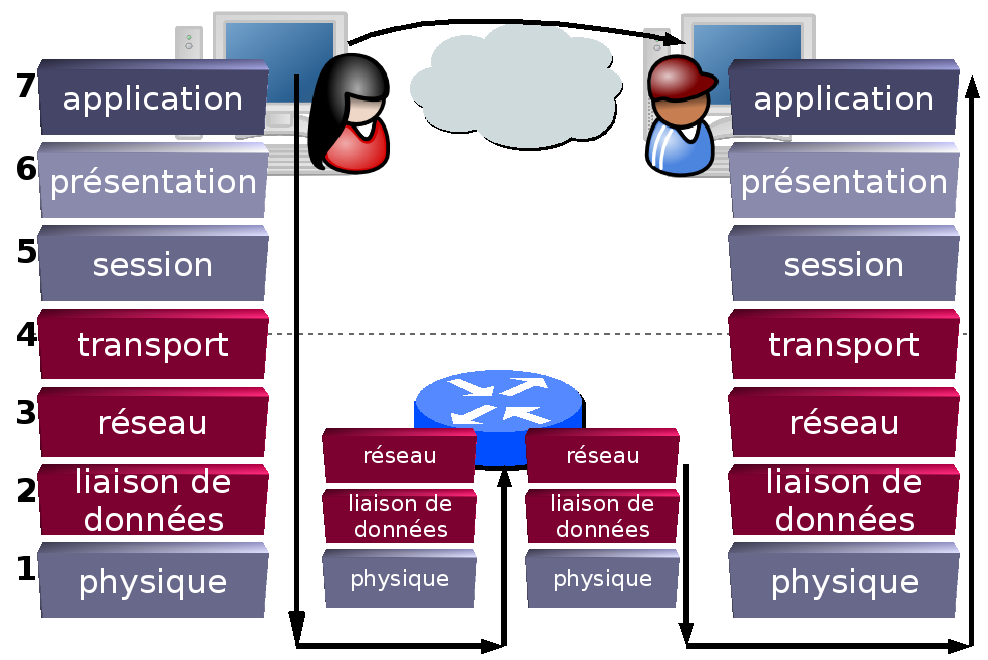
\includegraphics[width=13cm]{osi-model.png}
	\end{figure}
	\begin{description}
		\item[Application]
		\item[Présentation]
		\item[Session]
		\item[Transport] Contrôle de bout en bout
		\item[Réseau] Routage, IP, Adressage, contrôle de congestion
		\item[Liaison de données] Ethernet. Contrôle de flux, contrôle d'erreur
		\item[Physique] Transforme les données en signal
	\end{description}
	\begin{description}
		\item[Notion de service] la couche offre des services à la coche immédiatement supérieur en s'appuyant sur ceux offerts par celle immédiatement inférieure.
		\item[Notion d'encapsulation] Comment encapsuler le données venant de la couche supérieur pour --- les services offert à la couche
	\end{description}

	\chapter{Couche réseau}
	\section{Connexion}
	\begin{description}
		\item[Connexion] S'assurer de la présence du destinataire avant de communiquer
	\end{description}
	\begin{exemple}
		\begin{itemize}
			\item Le téléphone, celui-ci nécessite une connexion préalable. Les ressource sont réservées pour la communication sur les n\oe{}uds
				intermédiaires.
		\end{itemize}
	\end{exemple}

	\chapter{Couche transport}
	Le rôle de la couche transport est de transporter un message d'un équipement source vers un équipement destinataire et ce, de manière \textbf{fiable},
	\textbf{efficace} et \textbf{économique}.

	\begin{description}
		\item[fiable] Restitution de l'information dans l'intégralité.
		\item[Efficace] Rapide
		\item[Économique] En terme de bande passante et de ressource
	\end{description}

	La couche transport est la couche charnière entre les fonctions de traitement et les couches de transports de l'information. Elle masque aux
	applications les spécificités liées au réseau en leur offrant un service avec la qualité requise et en gérant efficacement les ressources.
	
	\section{Propriétés communes au transport}
	\subsection{Transport de bout en bout}
	La couche transport doit garantir l'acheminement du message, du source vers le de destinataire, éventuellement en traversant plusieurs réseau et en
	respectant la qualité de service requise par l'utilisateur.

	\subsection{Garantie de qualité de service}
	La couche transport se porte garant de la QoS\footnote{Quality of Service} fourni par la coche réseau, elle surveille et estime si elle est en
	mesure de respecter un ensemble de paramètre de QoS à savoir : 
	\begin{description}
		\item[Temps d'établissement de connexion] Durée qui s'écoule entre l'émission d'une demande et la confirmation de l'utilisateur.
		\item[Probabilité d'échec de la connexion] Mesure le risque qu'une connexion ne puisse s'établir dans un délais maximum défini.
		\item[Débit de la liaison] Donne le nombre d'octets utile qui peuvent être transférés en une seconde.
		\item[Temps de transit] Temps écoulé entre le moment ou l'utilisateur du service de transport envoie un message et celui ou l'entité de
			transport destinataire le reçoit effectivement.
		\item[Taux d'erreurs résiduel] Taux d'erreurs non corrigées qu'il est possible de rencontrer sur une connexion
		\item[Protection] Offre un maintient d'une sécurité pour éviter les manipulation non autorisées de données.
		\item[Priorité] Permettre de privilégier l'utilisation de différentes connexion par rapport à d'autre en cas de problème majeur.
		\item[Résiliation] Probabilité de déconnexion par la couche transport suite à un problème 
	\end{description}

	Ce sont es valeurs minimales, lors d'une demande d'établissement de connexion. La couche transport entre alors en phase de << Négociation >> de ces
	valeurs, soit d'un point de vue local, soit distant. Elle averti l'utilisateur des valeurs acceptés, ces valeurs demeurent inchangées durant toute
	la durée de la connexion.

	\subsection{Transparence des données échangées}
	Les données sont échangées sur une connexion transport indépendamment de leur format, de leur codage ou de leur signification, c'est le mode
	\textit{transparent}. L'avantage c'est qu'elle donne la possibilité au niveau transport de véhiculer des messages de taille quelconque, ce qui
	implique une gestion complexe de mémoire de stockage des données.

	\section{Les fonctionnalités du transport}
	Par certains aspects la couche transporta des fonctionnalités similaires de la couche liaison de données, comme le contrôleur d'erreur, le
	séquencement, le contrôle de débit. Cependant, il existe des différences fondamentales

	\begin{table}[H]
		\begin{tabular}{p{8cm}|p{8cm}}
			\textbf{Liaison de données} & \textbf{Transport}\\
			\hline
			Les entités communiquent via un canal physique.& Ce canal est remplacé par une interconnexion de réseau\\
			\hline
			Adressage & Adressage de destinataire plus compliqué\\
			\hline
			Établissement de la connexion simple &  Établissement de connexion plus compliqué\\
			\hline
			Mémorisation et contrôle de flux & Différentes approches dues à la gestion d'un nombre important de connexion. \\
			\hline
			& Errance des données
		\end{tabular}
		\end{table}

		\subsection{Établissement et libération de connexion}
	La vie d'une connexion de transport peut être divisé en trois phases
	\begin{description}
		\item[Établissement de la connexion] négociation des paramètre de QoS
		\item[Transfert de donnée sur cette connexion] 
		\item[Libération de la connexion]  fin de connexion reconnue par les deux extrémités
	\end{description}
	\subsection{Contrôle de flux et d'erreur et mémorisation}
	Le contrôle de flux consiste à réguler la transmission de données sans dépasser les possibilités de réception du destinataire.

	En cas de perte de message l'émetteur source doit mémoriser pour ré émettre.
	\subsection{Multiplexage éclatement}
	Un aspect pris en charge par la couche transport est l'optimisation des ressources réseau\footnote{En terme de cout et de performance} en fonction
	des besoin applicatifs.
	
	Le multiplexage est le partage d'une connexion réseau par plusieurs connexion transport et l'éclatement et l'utilisation de plusieurs connexion
	réseau pour une même connexion de transport.

	\subsection{Fragmentation et réassemblage}
	Les données applicatives ont parfois une taille importante\footnote{Comme par exemple lorsque l'application est une application de transfert de
	fichier}, étant donné la MTU du réseau local, le niveau transport doit fragmenter la donnée applicative pour qu'elle puisse être encapsulé sur le
	réseau local.

	\section{Adressage}
	Pour pouvoir communiquer avec ses correspondants le processus d'applications se met à l'écoute d'éventuels demande de connexion ou demande de
	transfert de données où il peut réaliser lui même ces transferts.
	Le niveau transport doit répéter ces différents processus afin d'aiguiller les données reçus lors des échanges. Ces repères sont appelés des points
	d'accès au service transport.

	Dans l'Internet ces points d'accès sont appelés des ports.

	L'adresse réseau sert à identifier de façon unique une machine sur le réseau tandis que le numéro de port identifie le processus d'application à
	laquelle les données sont destinés. Certains numéros de ports sont réservés pour des applications jouant le rôle de serveur. Ces numéros de ports peuvent être attribués dynamiquement

	\chapter{Les services et protocoles de l'Internet}
	Le réseau Internet s'appuie sur un réseau à 5 couches. 

	\begin{tabular}{p{8cm}|p{8cm}}
		\textbf{TCP} & \textbf{UDP}\\
		\hline
		Transport fiable d'un flux continu de données & transport non fiable\\
		\hline
		Service orienté connexion & Service non orienté connexion \\
		\hline
		Protocole complexe en terme de temps de réponse et lourd & Simple à mettre en oeuvre et débit plus importants\\
		\hline
		Mécanisme pour traiter les anomalies. Contrôle de flux et controle de congestion.& Aucun mécanisme\\
	\end{tabular}
	
	\section{Le service et le protocole TCP}
	Le service et le protocole tcp ont été conçue pour transporter de bout en bout des données de manières fiable, sur un ensemble de réseau non
	fiable. Cet ensemble de réseau se distingue à la grande hétérogénéité de ces composants en terme de topologie, de débit, de délais de transmission
	et de taille maximale de paquet.

	TCP s'adapte \textit{dynamiquement} a une variation et résiste à toute sorte de panne. Les données échangées sont considérés comme un flot de bits divises en
	octets, ces octets devant être reçue dans l'ordre dans lequel ils ont été reçus.

	\subsection{Les primitives du service TCP}
	\begin{description}
		\item[open] Permet de demander l'ouverture d'une connexion. En mode passif, l'utilisateur se positionne à l'écoute d'une demande de connexion.
			En mode actif l'utilisateur déclenche le dialogue avec l'entité distante en demandant l'établissement de cette connexion.
		\item[send] 
		\item[receive] Elle permet de recevoir un ensemble d'octets, récupérer les données dans le buffer, elle peut être blocante ou non selon le
			nombre d'octets disponible dans le buffer de réception.
		\item[close]  
		\item[status] Elle permet d'obtenir des informations d'états de la connexion. Comme par exemple l'identificateur du socket, l'état de la
			connexion, la valeur de la fenêtre de réception.
		\item[abort]  Permet d'interrompre la connexion avec la suppression de toutes les données en cours d'émission ou de réception
	\end{description}
	Pour avoir un service TCP, il faut créer deux extrémités  de connexion, l'un côtés source l'autre destinataire, ces extrémités sont appelés socket
	et correspondant à la combinaison adresse IP et numéro de port\footnote{Adresse ip sur 4 octets et numéro de port sur 2}

	La connexion est bidirectionnelle en mode point à point, on ne parle donc pas dans TCP de diffusion,celle-ci correspond à un flux d'octet.

	\subsection{Le protocole TCP}
	Les entités TCP s'échangent des TPDU appelés segment dont un entête de 20 octets fixes + une partie optionnel puis l partie données. Un segment TCP
	peut comporter jusqu'à $2^{16} = 65515$octets de données.

	Le protocole TCP utilise de base le principe de fenêtre d'anticipation, il arme un timer lorsque le segment arrive à destination, l'entité TCP
	réceptrice renvoit un segment sortant un numéro d'accusé de réception. 

	\subsubsection{Gestion de la Fiabilité}
		La retransmission du segment est déclenché par des temporisateur..

		\subsubsection{Calcul de la valeur de la temporisation}
		Cet algorithme à été proposé en 1988 par Jacobson.

		$RTT = (\alpha\times RTT_{estime} + (1-\alpha)\times NouveauRTT$ avec $0 \leq \alpha < 1$.

		Plusieurs échantillons sont nécessaire à partir de plusieurs segments transmis, il est calculé à partir de la formule ci-dessus avec le nouveau
		délai d'aller-retour observé et la valeur du RTT précédemment calculé.

		$RTO = \min\{BorneSuppRTO, \max\{borneInfRTO, RTO, RTT_{estime} \times \beta\}\}$ avec $\beta > 1$

		\begin{remarque}
			Cas particuliers du calcul d'aller:retour étant donné que l'ack reçu peut être soit celui du premier segment envoyé soit celui du second
			retransmis.
		\end{remarque}

		\paragraph{Cas particulier avec l'algorithme de Karn}
		TCP ne doit pas mettre à jour de RTT estimé dans le cadre de celui du segment retransmis.
		\subsubsection{Gestion de la congestion du réseau}
		Numéo en séquence codé sur 32bits, Raale de $2^{32}$octets.

		Conséquence d'un tel comportement: 
		\begin{enumerate}
			\item Encas d'erreur nombre élevé de retransmission
			\item Le récepteur peut être saturé
			\item Le réseau également
		\end{enumerate}

		Dans les échanges bidirectionnelles de TCP chaque émetteur annonce son crédit de nombre d'octets dans le champ fenêtre des segments qu'il
		envoi pour indiquer  le nombre d'octet qu'il est prêt à recevoir.

		Quand cette fenêtre est nulle, pas d'envoie de données de la part du correspondant sauf deux cas particulier : 
		\begin{itemize}
			\item Envoi possible de données d'urgences
			\item Envoi d'un segment contenant 1 seul octet pour obliger le correspondant à réannoncer le prochain octet attendu
		\end{itemize}<++>
\end{document}
 
